
\tcbuselibrary{theorems}
\tcbuselibrary{breakable, skins}
\tcbuselibrary{listings, documentation}
\geometry{
	a4paper,
	left=33mm,
	right=33mm,
	top=20mm}
% ========= Path to images ============
%   - Direct the computer on the path 
% 	  to the folder containg the images
% =====================================
\graphicspath{{./images/}}
% ============= Macros ================
\setlength{\parindent}{0pt}
\addto{\captionsenglish}{\renewcommand*{\contentsname}{Table of Contents}}
\linespread{1.1}
% ======== Footers & Headers ==========
\cfoot{\thepage}
\chead{}\rhead{}\lhead{}
% =====================================
\renewcommand{\thesection}{\arabic{section}}
\newcommand\sectionnumfont{% font specification for the number
	\fontsize{380}{130}\color{sectionNumbersColor}\selectfont}
\newcommand\sectionnamefont{% font specification for the name "PART"
	\normalfont\color{white}\scshape\small\bfseries }
% ========= Part Format ==========
\titleformat{\section}
{\normalfont\huge\filleft}
{}
{20pt}
{\begin{tikzpicture}[remember picture,overlay]
	\fill[sectionTitlesColor] 
	(current page.north west) rectangle ([yshift=-11cm]current page.north east);   
	\node[
	fill=frontPageColor,
	text width=2\paperwidth,
	text depth=18cm,
	anchor=center,
	inner sep=0pt] at (current page.north east) (parttop)
	{\thepart};%
	\foreach \i in {21,...,2}
	{
		\node[frontPageColor!95,rounded corners,draw,regular polygon,regular polygon sides=6, minimum size=\i cm,ultra thick] at ($(current page.north east)+(-21,0.15)$)
		{ ~ };
	}
	\node[
	anchor=south east,
	inner sep=0pt,
	outer sep=0pt] (partnum) at ([xshift=-20pt,yshift=5pt]parttop.south) 
	{\sectionnumfont\ifthenelse{\equal{\thesection}{0}}{}{\thesection}};
%	\node[
%	anchor=south,
%	inner sep=0pt] (partname) at ([yshift=2pt]partnum.south)   
%	{\sectionnamefont ~};
	\node[
	anchor=north east,
	align=right,
	inner xsep=0pt] at ([yshift=-0.5cm,xshift=9cm]current page.south|-partnum.south) 
	{{\MakeUppercase{\raggedleft#1}}};
	\end{tikzpicture}%
}
% ========= Hyper Ref ===========
\hypersetup{
	colorlinks,
	linkcolor={red!50!black},
	citecolor={blue!50!black},
	urlcolor={blue!80!black}
}
% ========= Boxed Notes ===========

\NewDocumentCommand\boxForNotes{m O{#1} O{grisfondo} O{primary} O{number within=section}} {
	\newtcbtheorem[#5]{#1}{#2} {
		enhanced,
		breakable,
		colback = #3,
		frame hidden,
		boxrule = 0sp,
		borderline west = {2pt}{0pt}{#4},
		sharp corners,
		detach title,
		before upper = \tcbtitle\par\smallskip,
		coltitle = #4,
		fonttitle = \bfseries\sffamily,
		separator sign none,
		segmentation style={solid, #4}
	}
	{th}
}

\boxForNotes{RemarkBlock}[\faInfoCircle~Remark][remarkBlockColor!12][remarkBlockColor]
\newcommand{\remarkBlock}[2]{\begin{RemarkBlock}{--- #1}{}#2\end{RemarkBlock}}

\boxForNotes{ExampleBlock}[\faChalkboardTeacher~Example][exampleBlockColor!12][exampleBlockColor]
\newcommand{\exampleBlock}[2]{\begin{ExampleBlock}{--- #1}{}#2\end{ExampleBlock}}

\boxForNotes{ReadBlock}[\faReadme~Suggested Reading][readBlockColor!12][readBlockColor]
\newcommand{\readBlock}[2]{\begin{ReadBlock}{--- #1}{}#2\end{ReadBlock}}

\boxForNotes{WarningBlock}[\faExclamationTriangle~Warning][warningBlockColor!12][warningBlockColor]
\newcommand{\warningBlock}[2]{\begin{WarningBlock}{--- #1}{}#2\end{WarningBlock}}

\boxForNotes{CuriosityBlock}[\faQuestionCircle~Curiosity][curiosityBlockColor!12][curiosityBlockColor]
\newcommand{\curiosityBlock}[2]{\begin{CuriosityBlock}{--- #1}{}#2\end{CuriosityBlock}}




\newcommand{\notes}[3]{
{
	\addcontentsline{toc}{section}{NOTES ON #1}
}
%{\newpage ~ \clearpage}
\begin{tikzpicture}[remember picture,overlay]
	\thispagestyle{empty}
	%%%%%%%%%%%%%%%%%%%% Background %%%%%%%%%%%%%%%%%%%%%%%%
	\fill[white] (current page.south west) rectangle (current page.north east);
	
	
	\foreach \i in {0.5,...,22}
	{
		\node[rounded corners,frontPageColor!25,draw,regular polygon,regular polygon sides=6, minimum size=\i cm,ultra thick] at ($(current page.west)+(2.5,-5)$) {} ;
	}
	
	%%%%%%%%%%%%%%%%%%%% Background Polygon %%%%%%%%%%%%%%%%%%%% 
	\foreach \i in {0.5,...,22}
	{
		\node[rounded corners,frontPageColor!20,draw,regular polygon,regular polygon sides=6, minimum size=\i cm,ultra thick] at ($(current page.north west)+(2.5,0)$) {} ;
	}
	
	\foreach \i in {0.5,...,22}
	{
		\node[rounded corners,frontPageColor!10,draw,regular polygon,regular polygon sides=6, minimum size=\i cm,ultra thick] at ($(current page.north east)+(0,-9.5)$) {} ;
	}
	
	
	\foreach \i in {21,...,2}
	{
		\node[frontPageColor!15,rounded corners,draw,regular polygon,regular polygon sides=6, minimum size=\i cm,ultra thick] at ($(current page.south east)+(-0.2,-0.45)$) {} ;
	}
	
	\node[align=center,frontPageColor!95,minimum width=0.625*\paperwidth,minimum height=3cm, rounded corners] at ($(current page.north)+(0,-8)$)
	{
		{\fontsize{30}{30} \selectfont \bfseries #1}
	};
	
	\node[align=center,frontPageColor!90,minimum width=0.625*\paperwidth,minimum height=2cm, rounded corners] at ($(current page.north)+(0,-6.5)$)
	{
		{\fontsize{20.75}{30} \textit{Notes on}}
	};

	\node[align=center,black!95,minimum width=0.625*\paperwidth,minimum height=2cm, rounded corners] at ($(current page.north)+(6,-26.55)$)
	{
		{\textit{#2}}
	};

	\node[align=center,black!95,minimum width=0.625*\paperwidth,minimum height=2cm, rounded corners] at ($(current page.north)+(6,-27.4)$)
	{
		{\textit{#3}}
	};
		
\end{tikzpicture}
{\glsresetall}
{\newpage}
}



% title background image
\backgroundsetup{
	scale=1,
	angle=0,
	position=current page.center,
	opacity=0.12, % adjust: smaller = whiter/less visible
	contents={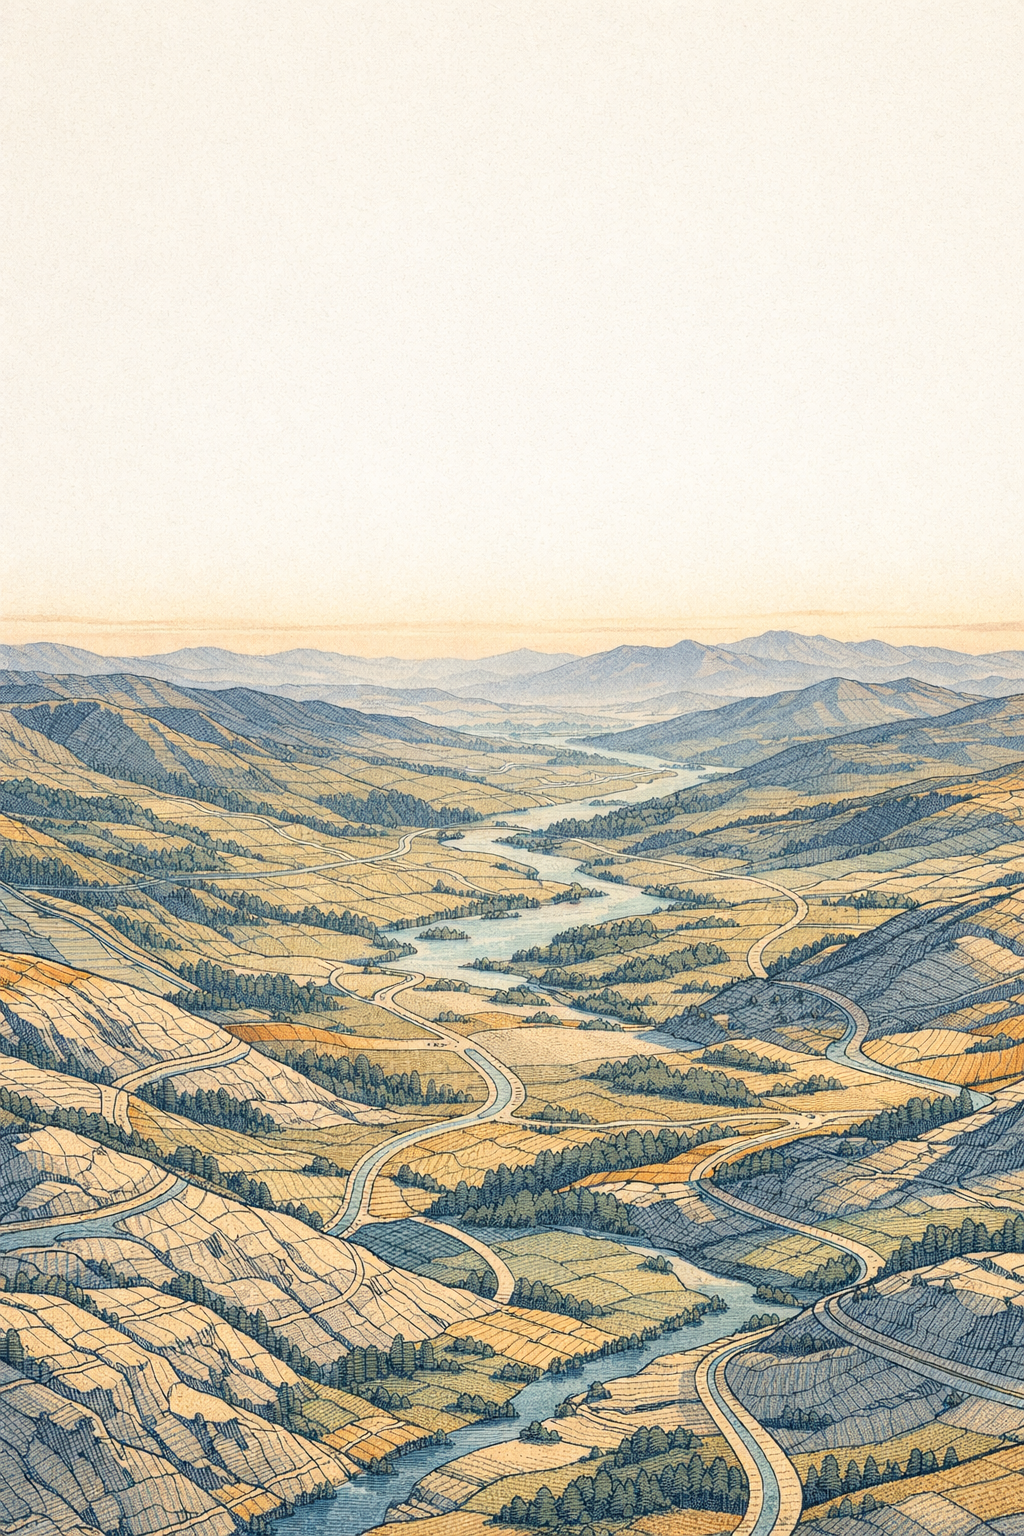
\includegraphics[width=\paperwidth,height=\paperheight]{resources/img/background.png}}
}